\chapter{Performance Testing and User Perception}
\label{cha:performance}

The research question of the thesis is if \emph{React} can be combined with \emph{D3} without losing any performance in the browser. The following sections introduce the reader not only to the benchmark setup and testing methodologies but also present the final results of the benchmarks. There is also a discussion which elaborates all test results. Since humans cannot measure the exact amount of frames per second, a special section introduces the reader to the human perception of fluent animations and how the testing results can be interpreted even further with that knowledge.

\section{Test Environment Setup}

This section describes the testing environment that was implemented to compare the three force simulation component prototypes. There are a few challenges that had to be taken into account when realizing the testing environment. Also, the implementation details are elaborated and explained. Last but not least, the testing devices are introduced which are used to run the benchmark.

\subsection{Challenges}

One of the most challenging aspects of the thesis project is the performance measurement of the prototypes. Modern browsers have an uncountable amount of features that help to smooth out the performance to improve user perception. Getting some consistent performance numbers is much harder due to inconsistent browser optimizations. Using different browsers for benchmarks also means that different \emph{JavaScript} runtimes are used to run the benchmarks. All engines have different execution and parsing speeds. Also, the mechanism to speed up frequently accessed script code is different, which also makes it harder to get consistent performance numbers.

When benchmarking web applications, it is very complicated to get performance values that have scientific relevance, which can be compared to get some accurate results. The next section introduces a system that was primarily implemented to measure the performance of \emph{JavaScript} web applications. The system tries to tackle all challenges to producing detailed benchmark results.

Another big problem is the fact that browsers detect the refresh rate of monitors when utilizing the request animation frame functionality. Monitors with a refresh rate of 144 Hertz allow browsers to produce up to 144 frames per second. 60-Hertz monitors, on the other hand, limit the browser's framerate to 60 FPS. The maximum amount of animation frame executions in any browser can only ever go up to the monitor's amount of Hertz the browser window is running in. 

Speaking of utilizing the request animation frame functionality, it must be mentioned that each browser has a different implementation of the functionality. The \emph{Chrome}\footnote{\url{https://www.google.com/intl/de/chrome/}} browser, for example, is smoothing out the performance by trying to execute animation frames regularly, which means that the overall performance might be lowered to achieve a smoother framerate as explained in~\cite{ChromeRAF}. Experience shows that \emph{Firefox}\footnote{\url{https://www.mozilla.org/de/firefox/new/}}, on the other hand, always fires its animation frames whenever a frame is available, which can result in higher overall but not as consistent framerates.

Last but not least, another challenge was to build a performance measuring environment that can be used without adding code to the prototypes. Theoretically, each prototype should be a complete component that can be shipped as a third party library. By adding performance measurement specific code, the components would contain functionality that is not needed when shipping production builds of the components.

\begin{figure}
  \centering
  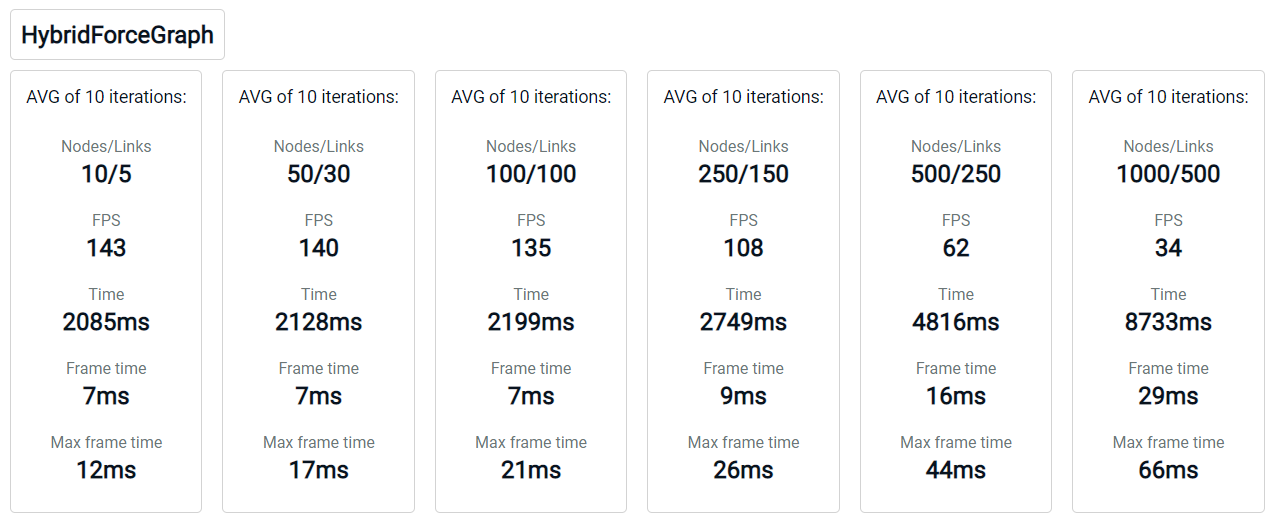
\includegraphics[width=1\columnwidth]{testresults}
  \caption{Hybrid prototype benchmark results.}
  \label{fig:reactD3benchResult}
\end{figure}

\subsection{Building a Stable Testing Environment}
\label{sub:perfImplDetails}

A testing environment which produces consistent data input across multiple iterations yields the best testing results when benchmarking all three prototypes. Testing the force simulation prototypes with the same data across multiple benchmarks, environments, and devices is of utmost importance. A valid solution is to use a pseudo-random data generator which can be restarted and reseeded each benchmark iteration.

Generating an arbitrary amount of random node and link positions is not a problem, as \emph{JavaScript} has a built-in random generator which can be utilized to generate random data. Unfortunately, \emph{JavaScript's} random generator cannot be seeded to achieve consistent pseudo-random results. The library \emph{seedrandom} in~\cite{SeedRandom} is the perfect technology to solve the problem of generating consistent data across multiple iterations of the benchmark tests.

Since browsers frequently yield different performance numbers across iterations with identical data, the amount of cycles per test data iteration has to be increased. When testing one specific iteration multiple times, the average value has much more significance than testing an iteration only once. Therefore the testing environment must have support for different iteration configurations, which can be run an arbitrary amount of times.

\begin{figure}
  \centering
  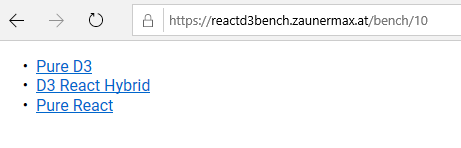
\includegraphics[width=0.5\columnwidth]{reactd3bench}
  \caption{Overview of the benchmark application.}
  \label{fig:reactD3bench1}
\end{figure}

The testing environment is designed to be a stateful container which generates some random data and then passes it to the desired prototype. \emph{D3} simulations provide a mechanism to add an event handler whenever the simulation stops. Therefore, it is no problem to pass a handler to the benchmark component that is executed whenever the simulation stops. The handler can be used to restart the benchmark with some newly generated data until the desired amount of benchmark iteration cycles is reached.

Pseudo-randomly generated data is obtained by a specially implemented custom helper utility module. The custom module is designed to generate a specified amount of random nodes and links. The method to generate random data takes two parameters---the number of nodes and the number of links. Generating consistent pseudo-random data is possible by internally using the previously mentioned seedrandom module.

Tackling the performance measurement problem is a much harder task, however. To be able to measure the number of frames per second, the request animation browser functionality can be used. Another custom implemented module provides some functionality that is specifically designed to measure performance intensive \emph{JavaScript} animations. By requesting an animation frame as often as possible in a terminable infinite loop, a reference timestamp can be used to measure the amount of animation frame executions per second which is equal to the frames per second the browser produces.

Presenting the performance results must not be underestimated either. To provide benchmark results appealingly, each iteration is represented via a visual container that contains all relevant information for a specific test iteration. If there are six test iterations, six containers are rendered after the benchmark. The containers contain the number of cycles per iteration, the test configuration, the number of frames per second, the overall execution time per cycle, the average frame time, and also the highest frame time. Figure~\ref{fig:reactD3benchResult} shows how the benchmark results visually look like.

Finally, the benchmark tool has to be easy to use on all kinds of devices. The thesis project also contains a small \emph{React} application which can be deployed on any static web hosting service that can serve single page applications. A visual representation of the basic benchmark app can be seen in figure~\ref{fig:reactD3bench1}. The \emph{React} application is a wrapper around the testing environment, which lets users select the desired benchmark for any of the three force simulation prototypes and then runs it in the browser. Each benchmark also has an easily distinguishable URL to be able to copy paste a specific benchmark URL into any browser. Figures~\ref{fig:reactD3bench1} and~\ref{fig:reactD3bench2} show how the URL contains all relevant benchmark parameters. That way the benchmark URLs can be pasted into any browser to execute the benchmark. 

\begin{figure}
  \centering
  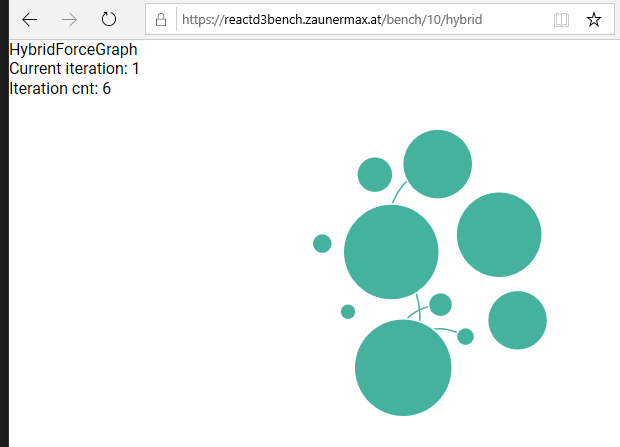
\includegraphics[width=0.6\columnwidth]{reactd3bench1}
  \caption{The benchmark currently iterating through hybrid prototype iterations.}
  \label{fig:reactD3bench2}
\end{figure}

\section{Testing Setup}

Having a bulletproof testing setup plays a fundamental role in producing scientifically releveant test results. Therefore, the following sections of the thesis provide a thorough insight into the testing devices and on how the whole benchmark methodology is conceptionalized. 

\subsection{Testing Devices}

\begin{table}
  \centering
  \begin{threeparttable}
    \caption{The table shows a list of low-end testing devices.}
    \label{tab:lowendTestingDevices}
    \centering
    \def\rr{\rightskip=0pt plus1em \spaceskip=.3333em \xspaceskip=.5em\relax}
    \setlength{\tabcolsep}{1ex}
    \def\arraystretch{1.20}
    \setlength{\tabcolsep}{1ex}
    \small
    \begin{english}
      \begin{tabular}{|c||c|c|c|}
        \hline
          \multicolumn{1}{|c||}{\emph{Device}}&
          \multicolumn{1}{|c}{\emph{CPU}} &
          \multicolumn{1}{|c}{\emph{GPU}} &
          \multicolumn{1}{|c|}{\emph{RAM}} \\
        \hline
        \hline
        OnePlus 1 & 
        Snapdragon 801 & 
        Adreno 330 & 
        3GB \\
        \hline
        OnePlus 5T & 
        Snapdragon 835 & 
        Adreno 540  & 
        8GB \\
        %%\hline
        %%Samsung G\tnote{1} \hspace{0.1mm} S8 & 
        %%Exynos 8895 & 
        %%Mali-G71 MP20 & 
        %%4GB \\
        %%\hline
        %%Samsung GT\tnote{2} \hspace{0.1mm} A10.1 &
        %%Exynos 7870 & 
        %%Mali-T830 MP2 & 
        %%3GB \\
        \hline
        SurfaceBook & 
        Intel i5-6300U & 
        Intel HD 520 & 
        8GB \\
        \hline
      \end{tabular}  
    \end{english}
    %%\begin{tablenotes}
    %%\item [1] Galaxy
    %%\item [2] Galaxy Tab
    %%\end{tablenotes}
  \end{threeparttable}
\end{table}

The amount of test devices should be as high as possible while still being reasonable regarding to the effort it takes to process all resulting benchmark data. A total amount of six devices is enough to retrieve scientifically sig\-nifi\-cant results because each prototype is not only tested on each device, but also on two browsers with multiple iteration difficulties which are executed multiple times. The range of devices is divided into two sections: high-end devices and low-end devices. 

The mobile devices used for testing are a \emph{OnePlus 1} phone, a \emph{OnePlus 5t} phone, and a \emph{SurfaceBook} in tablet mode. All low-end devices and their specs are listed in table~\ref{tab:lowendTestingDevices}. It must be noted that every selected low-end device has a monitor refresh rate of 60-Hertz. 

Table~\ref{tab:highendTestingDevices} introduces all high-end devices which have a monitor refresh rate of 144-Hertz. Two of the listed devices are custom tower builds with custom specs and one device is a \emph{Razer Blade 15} laptop with specs defined by its manufacturer. All in all the devices should provide a good overview of the performance of the force graph components.

\begin{table}
  \centering
  \begin{threeparttable}
    \caption{The table shows a list of high-end high refresh rate testing devices.}
    \label{tab:highendTestingDevices}
    \centering
    \def\rr{\rightskip=0pt plus1em \spaceskip=.3333em \xspaceskip=.5em\relax}
    \setlength{\tabcolsep}{1ex}
    \def\arraystretch{1.20}
    \setlength{\tabcolsep}{1ex}
    \small
    \begin{english}
      \begin{tabular}{|c||c|c|c|c|}
        \hline
          \multicolumn{1}{|c||}{\emph{Device}}&
          \multicolumn{1}{|c}{\emph{CPU}} &
          \multicolumn{1}{|c}{\emph{GPU}} &
          \multicolumn{1}{|c|}{\emph{RAM}} \\
        \hline
        \hline
        Tower (Max Z.) & 
        Intel i9-7900X & 
        2x Nvidia GTX 1080Ti & 
        32GB \\
        \hline
        Razer Blade 15 (2018) & 
        Intel i7-8750H & 
        Nvidia GTX 1070 Max-Q  & 
        16GB \\
        %%\hline
        %%Tower (Max J.) & 
        %%Intel i7-7700k & 
        %%Nvidia GTX 1070 & 
        %%16GB \\
        \hline
        Tower (Patrick M.) &
        Intel i7-6700k & 
        Nvidia GTX 1080 & 
        16GB \\
        %%\hline
        %%Tower (Julian J.) & 
        %%Intel i7-7700k & 
        %%Nvidia GTX 1070 & 
        %%16GB \\
        \hline
      \end{tabular}  
    \end{english}
  \end{threeparttable}
\end{table}

\subsection{Testing Methodologies}

\begin{figure}
\centering
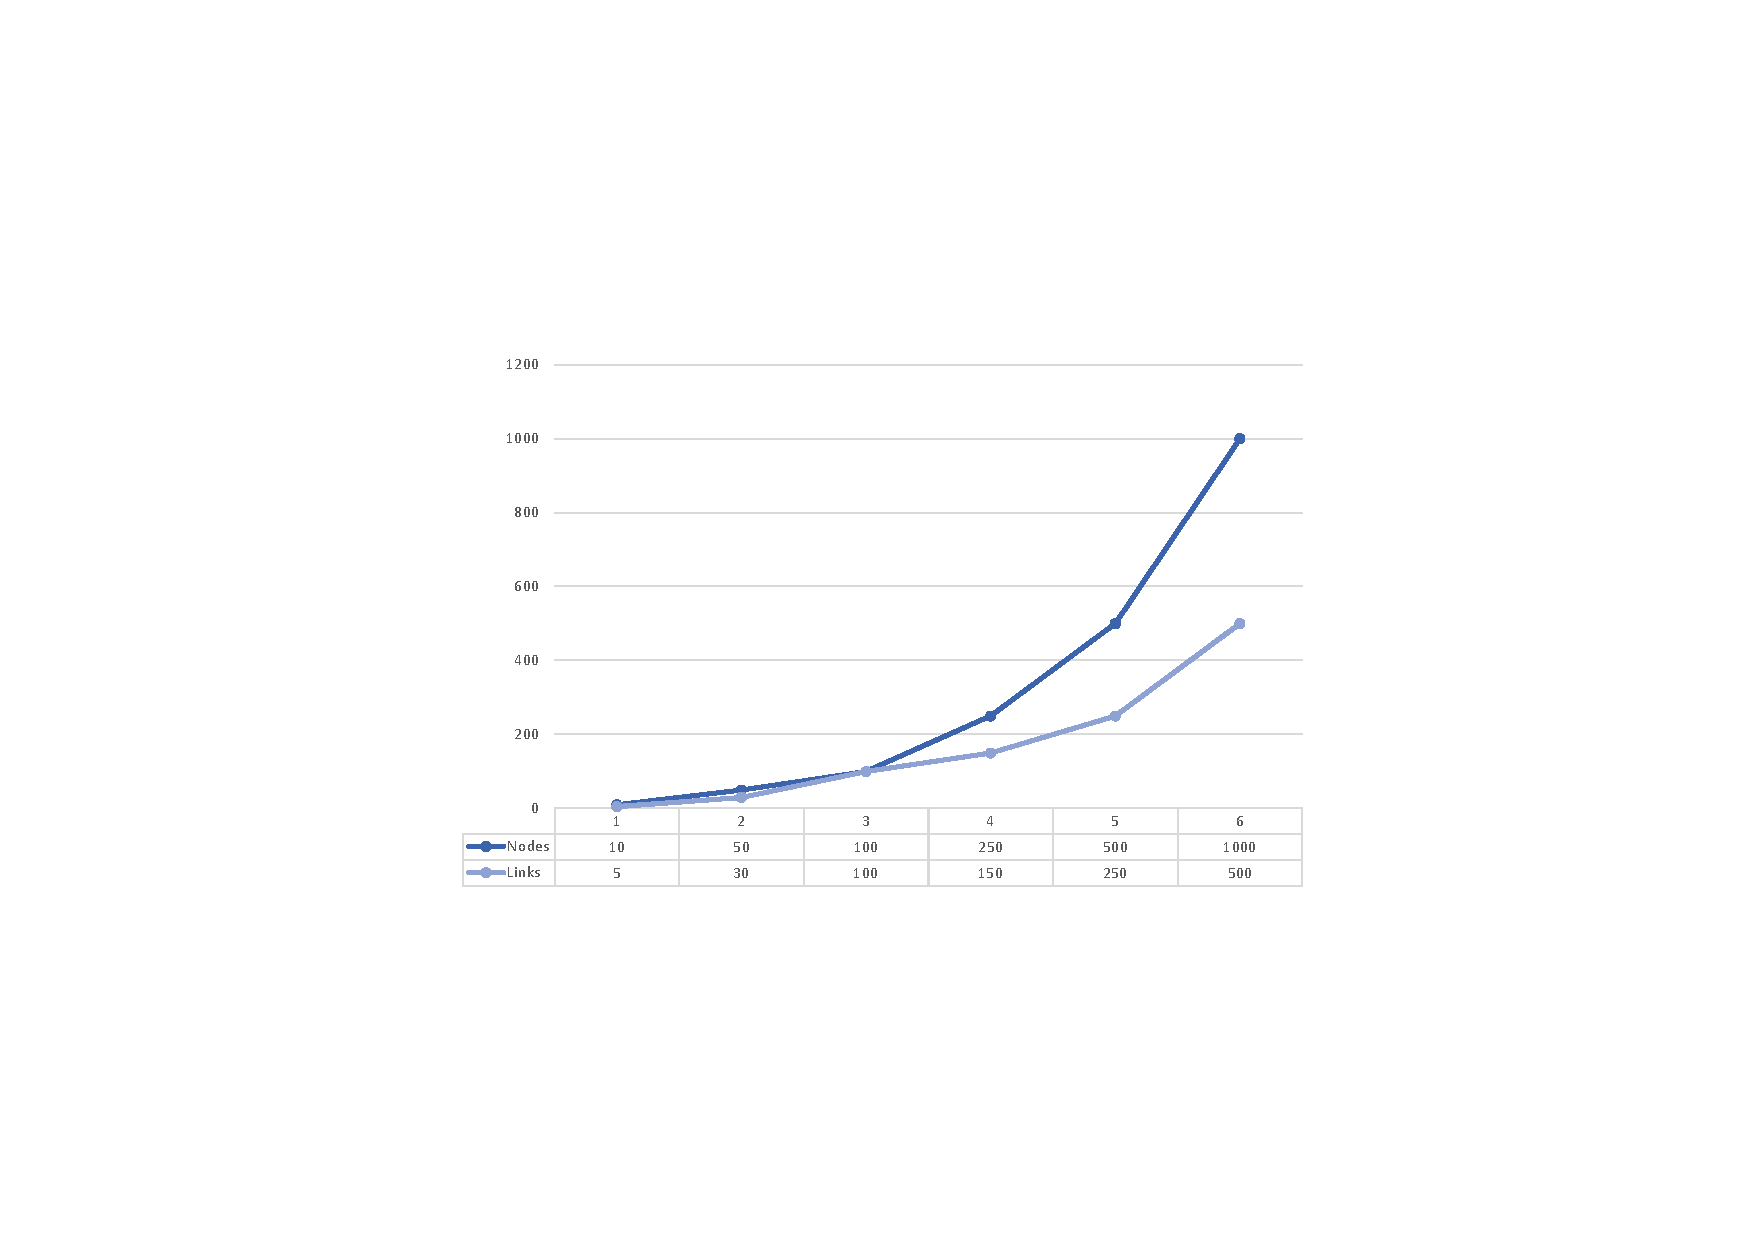
\includegraphics[scale=2.5, trim= 4cm 5cm 4cm 5cm, clip, width=1\columnwidth]{perfIterations.pdf}
\caption{Benchmark iteration configuration.}
\label{fig:perfIterations}
\end{figure}

Running the benchmarks to get good quality testing results is relatively straight forward. To get the most declarative performance numbers it is best to mainly use devices with a high monitor refresh rate. Devices with a low monitor refresh rate can possibly falsify some testing results. If, for example, a browser could possibly render 100 frames per second during an iteration, a system with a 60-Hertz monitor would only be able to measure a maximum of 60FPS as the theoretically possible 100 FPS would be capped to the monitor's 60-Hertz refresh rate.

Devices with high refresh rates can be sufficient for measuring the overall best performing prototype. One of the more interesting research aspects of the thesis though is the question, how well the prototypes perform on mobile devices with lower performance specifications than desktop PCs. Thus the testing results must be split up into different categories as a consequence. Due to the fact that not only frames per second, but also other perfromance aspects like total execution time are measured, the lower performing devices can also be compared to each other.

Each device runs through six iterations per prototype with exponentially increasing rendering difficulty. Figure~\ref{fig:perfIterations} shows the benchmark configuration for the benchmark. Starting with a node count of 10 and a link count of five, the configuration ultimately goes up to 1000 nodes and 500 links. The third iteration is special, as the number of nodes and links is the same. The special configuration was added to test an extreme scenario of all nodes being connected to each other to induce some extra performance heavy force calculations.

Each iteration runs through 10 cycles which equals to a grand total of 60 cycles per prototype, browser, and device combination. Three high-end devices with 144-Hertz monitors and the three low-end devices with 60-Hertz monitors run the benchmark iterations in the \emph{Chrome} and in the \emph{Firefox} browser. The two browsers were selected, because they are the most sig\-nifi\-cantly used, platform independent browsers worldwide according to the statistics in~\cite{StatCounterBrowserMarketShare} and~\cite{W3CBrowserMarketShare}. Taking into account that there are six devices, three prototypes, and two browsers, the total number of iterations is 36.

\section{Benchmark Results}

This section answers the research question if \emph{React} can be combined with \emph{D3} without introducing any performance losses in the browser. Extensive benchmark testing sessions resulted in some remarkable research results which are presented below. After presenting the test results, an introduction to the human perception of fluent animations helps the reader to follow the subsequent interpretation of the benchmark results.

\subsection{Introducing the Test Results}

First of all, the thesis project is a success, as the overall performance numbers show a clear trend that the hybrid prototype is ahead of \emph{Uber's} pure react implementation. The total execution time of all combined benchmark iteration cycles is exactly 25326s when combining the average execution times of each test. When converting milliseconds to hours, the result is 7.04 hours. Since the benchmark environment was designed for extensive benchmark sessions, the time between running the benchmarks was minimized. The only manual task was to write down the actual benchmark results. Letting devices run the tests required no further user interaction. 

Figure~\ref{fig:perfLowEnd001} shows the average FPS of the low-end devices. An overall downwards trend can immediately be seen in the FPS chart, which is expected. The more DOM nodes the browsers have to calculate, the lower the frames per second get per iteration. Each group of bars in the chart represents an average value for each prototype per benchmark iteration. Note that all values are the average taken from 10 iteration cycles of the \emph{Chrome} and the \emph{Firefox} browser. The prototypes mostly yielded the expected performance numbers starting with the reference performance of the pure \emph{D3} prototype, followed by the hybrid component and then finally followed by the pure \emph{React} force graph component.

\begin{figure}
\centering
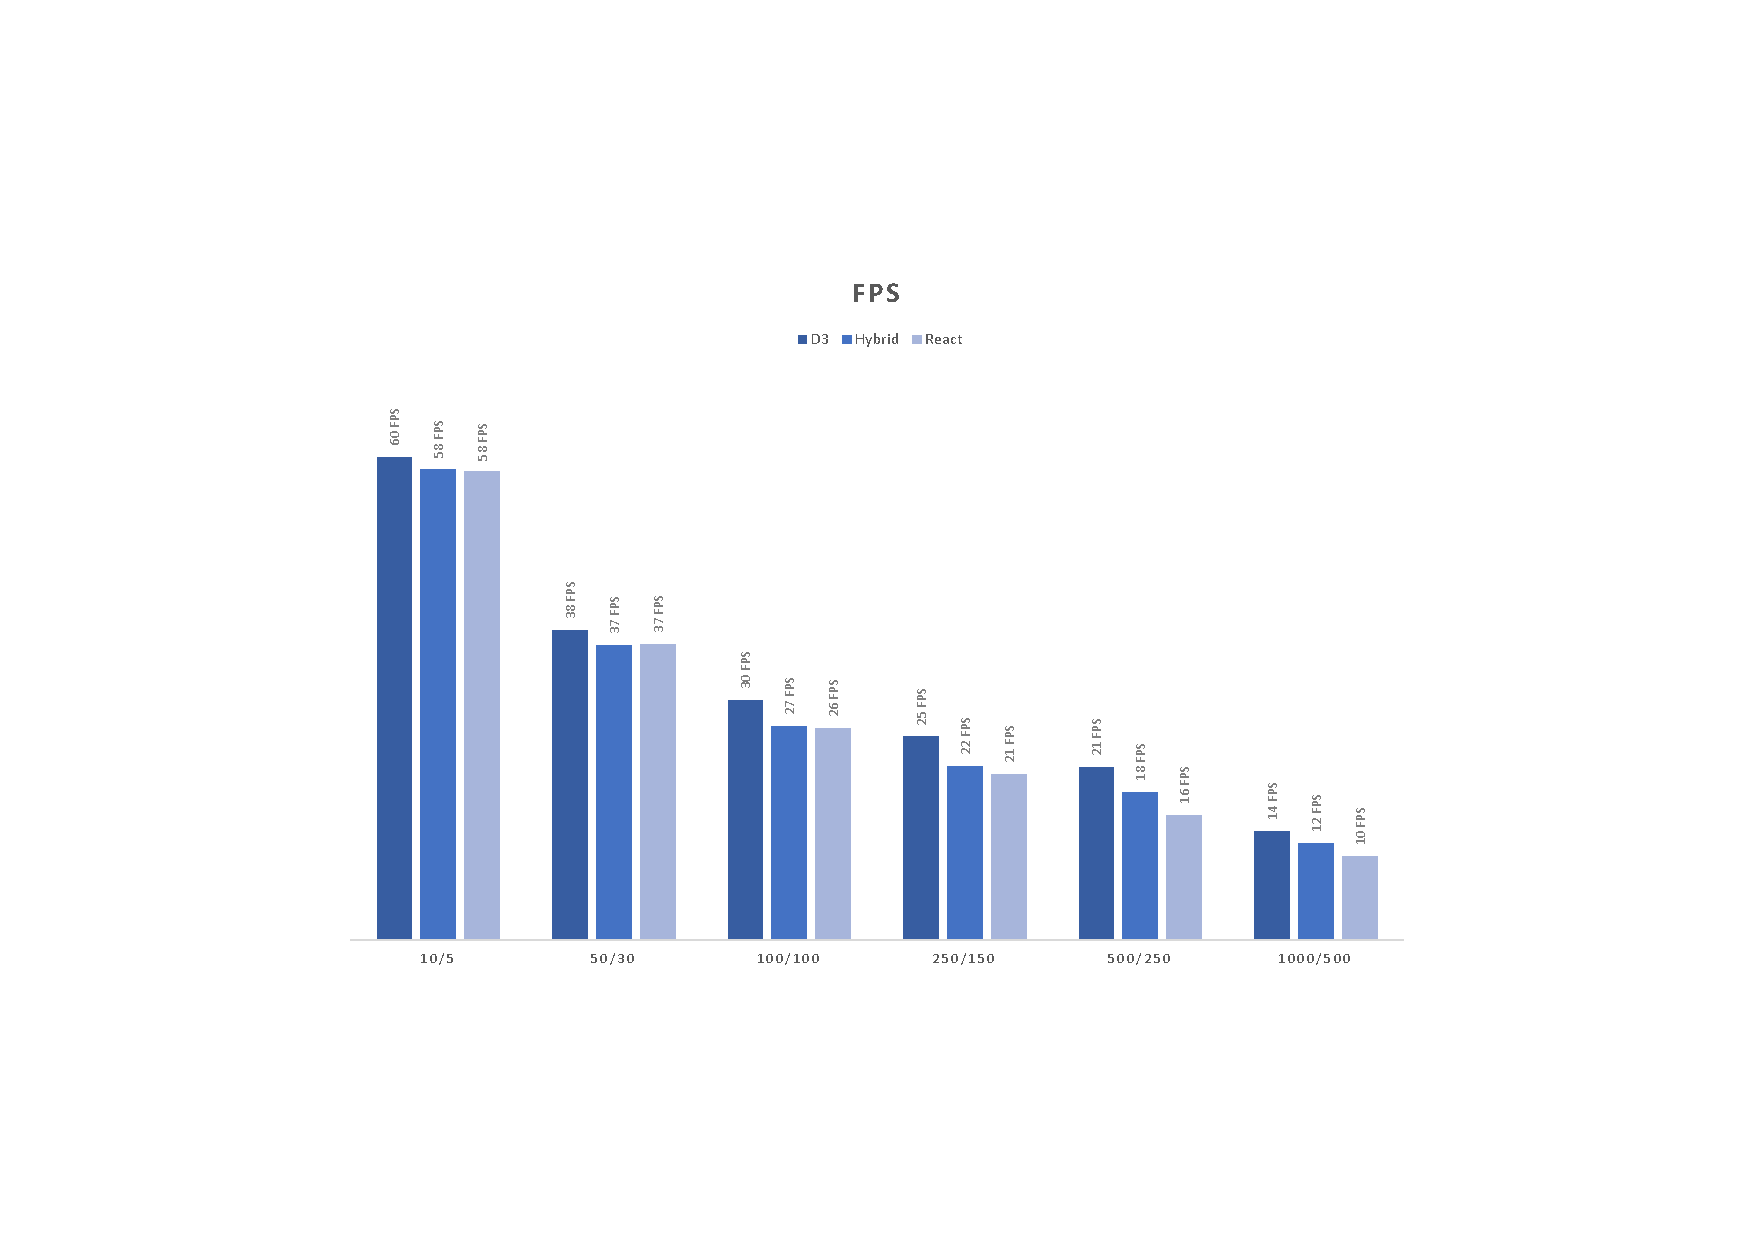
\includegraphics[scale=2.5, trim= 4cm 4.5cm 4cm 4.5cm, clip, width=1\columnwidth]{perfLowEnd001.pdf}
\caption{Low-end devices' average frames per second per benchmark iteration cycle (higher is better).}
\label{fig:perfLowEnd001}
\end{figure}

Figure~\ref{fig:perfHighEnd001} shows the average FPS values of the high-end devices' benchmark iterations. Looking at the bar chart, it is apparent that the high-end devices hit the FPS cap of 144 FPS throughout the first few iteration cycles. From the third iteration a steady decrease of FPS can be observed though, as the iteration difficulty is high enough for all devices not to hit the monitor refresh rate limit anymore.

\begin{figure}
\centering
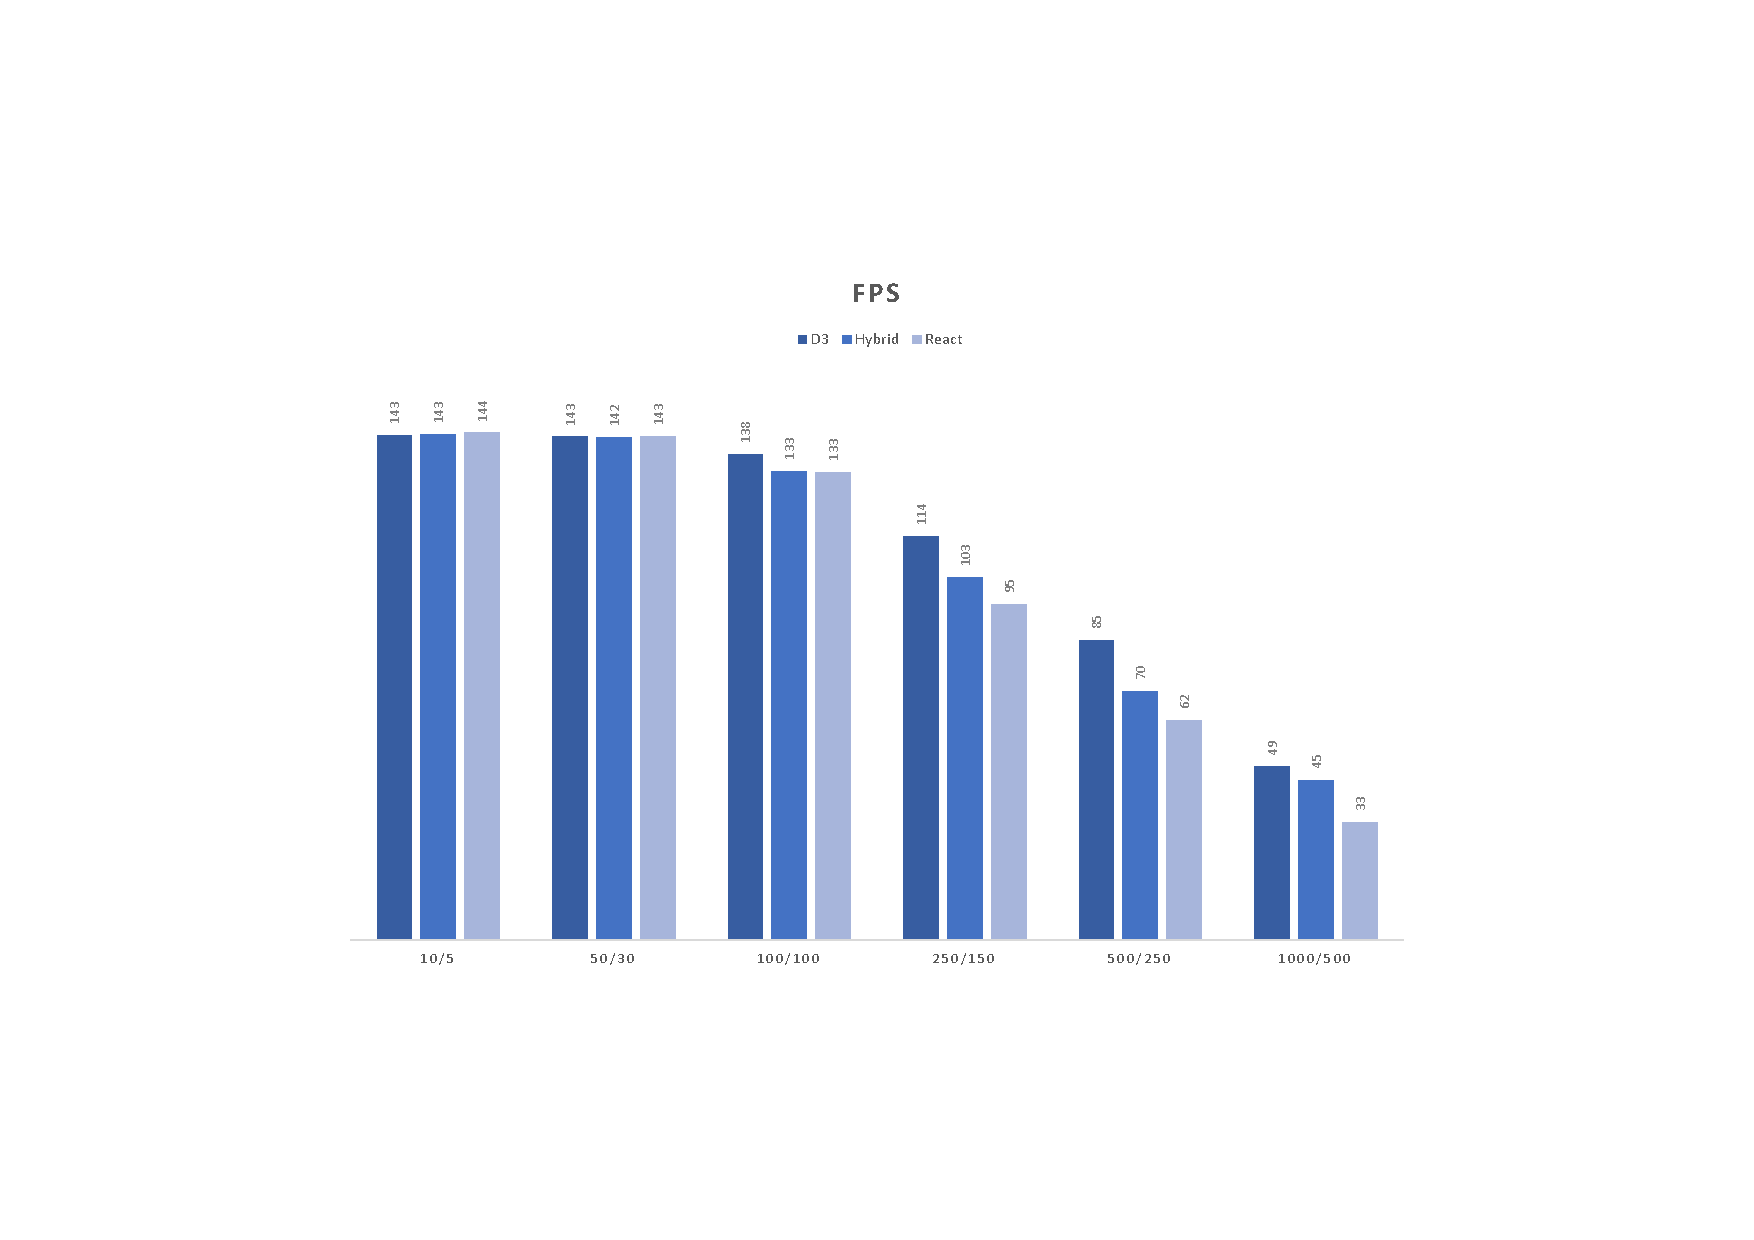
\includegraphics[scale=2.5, trim= 4cm 4.5cm 4cm 4.5cm, clip, width=1\columnwidth]{perfHighEnd001.pdf}
\caption{High-end devices' average frames per second per benchmark iteration cycle (higher is better).}
\label{fig:perfHighEnd001}
\end{figure}

The bar chart in figure~\ref{fig:perfLowEnd002} shows the average time it took to complete the benchmark fully. Via the browsers' performance API, exact timestamps can be measured once a benchmark cycle starts, and once it ends. By subtracting the start timestamp from the end timestamp the overall time to execute is calculated. Like the FPS chart, the time to complete (TTC) chart also shows all average values it took the different prototypes to complete the benchmark cycles.

\begin{figure}
\centering
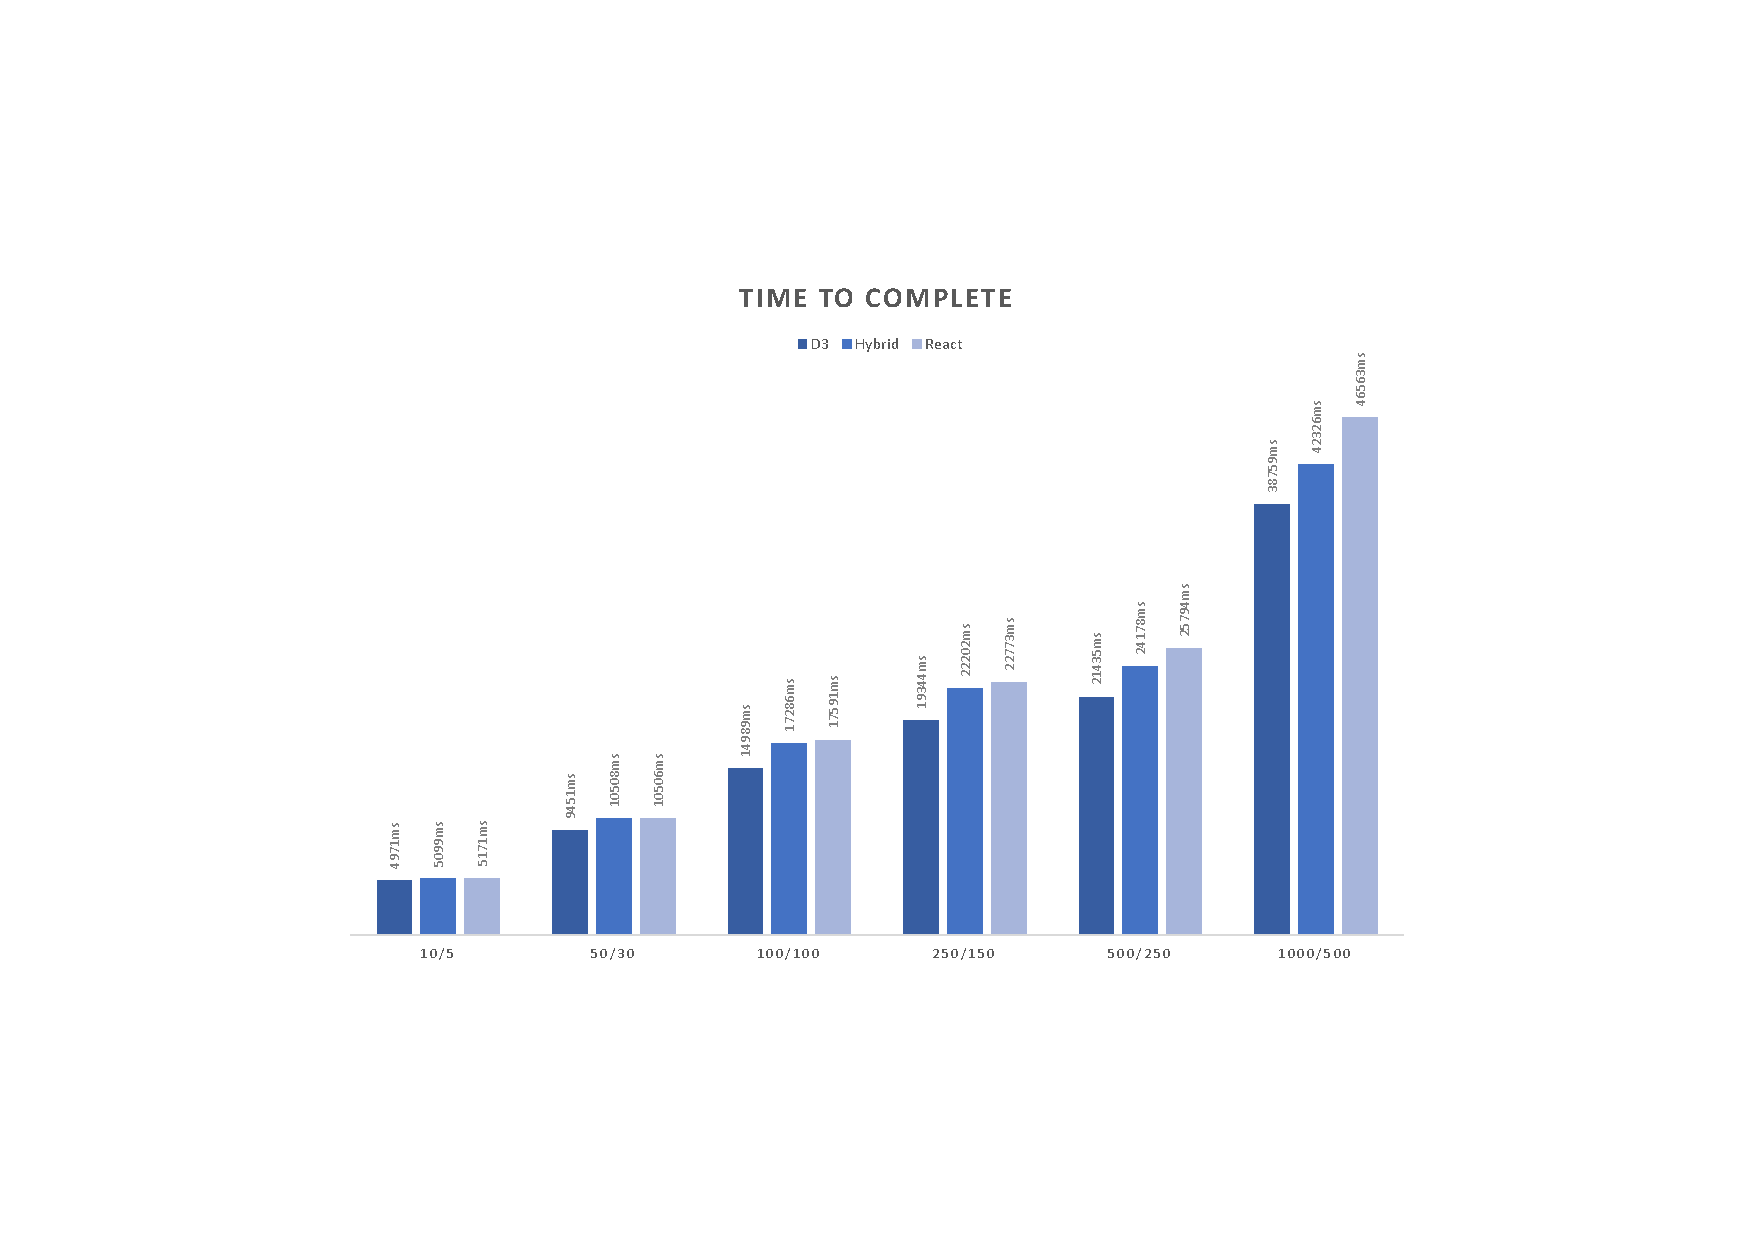
\includegraphics[scale=2.5, trim= 4cm 4.5cm 4cm 4.5cm, clip, width=1\columnwidth]{perfLowEnd002.pdf}
\caption{Low-end devices' average time to complete for one benchmark iteration cycle in milliseconds (lower is better).}
\label{fig:perfLowEnd002}
\end{figure}

Continuing with the high-end devices, the chart in figure~\ref{fig:perfHighEnd002} shows the average time in milliseconds it took the devices to finish one iteration cycle. The results show that not only FPS can be capped at maximum values but also the TTC can be capped at a minimum value as shown in the first iteration cycles. Since the performance measurement utility is tied to the browsers' animation frame functionality, being capped at a maximum value also means being restricted on minimum values.

\begin{figure}
\centering
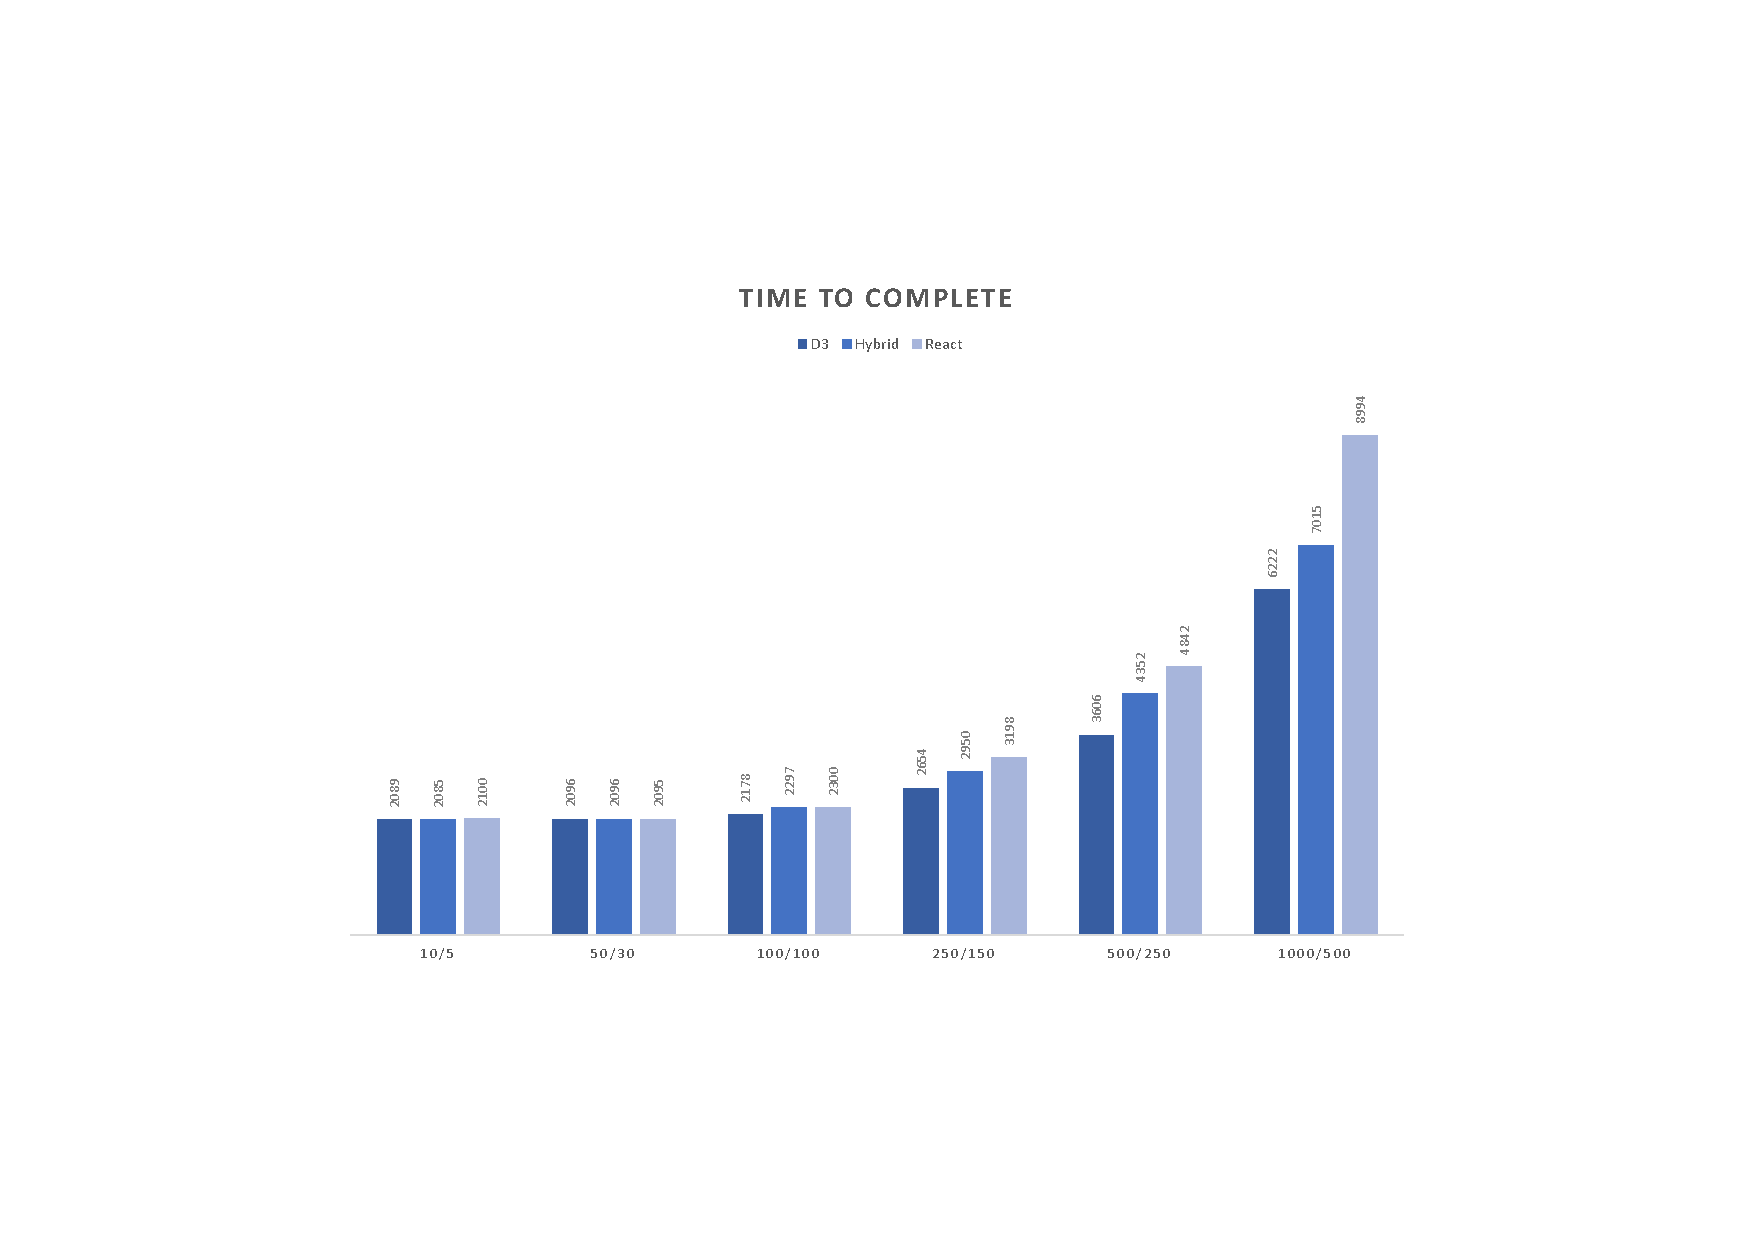
\includegraphics[scale=2.5, trim= 4cm 4.5cm 4cm 4.5cm, clip, width=1\columnwidth]{perfHighEnd002.pdf}
\caption{High-end devices' average time to complete for one benchmark iteration cycle in milliseconds (lower is better).}
\label{fig:perfHighEnd002}
\end{figure}

%% frametime another way to display frames per second, just another calculation

Measuring the average frame time of animations can provide insights into the user's perception of fluent animation. If the value is too high, the animation may not be experienced as a smooth animation. Therefore measuring the value is crucial when comparing the prototypes to each other. Figure~\ref{fig:perfLowEnd003} shows a bar chart of the low-end device benchmark. Towards the last two iterations, the benchmark configuration seems to have hit a certain threshold since the values rise exponentially. The other performance results show a similar pattern to the previous results, however.

\begin{figure}
\centering
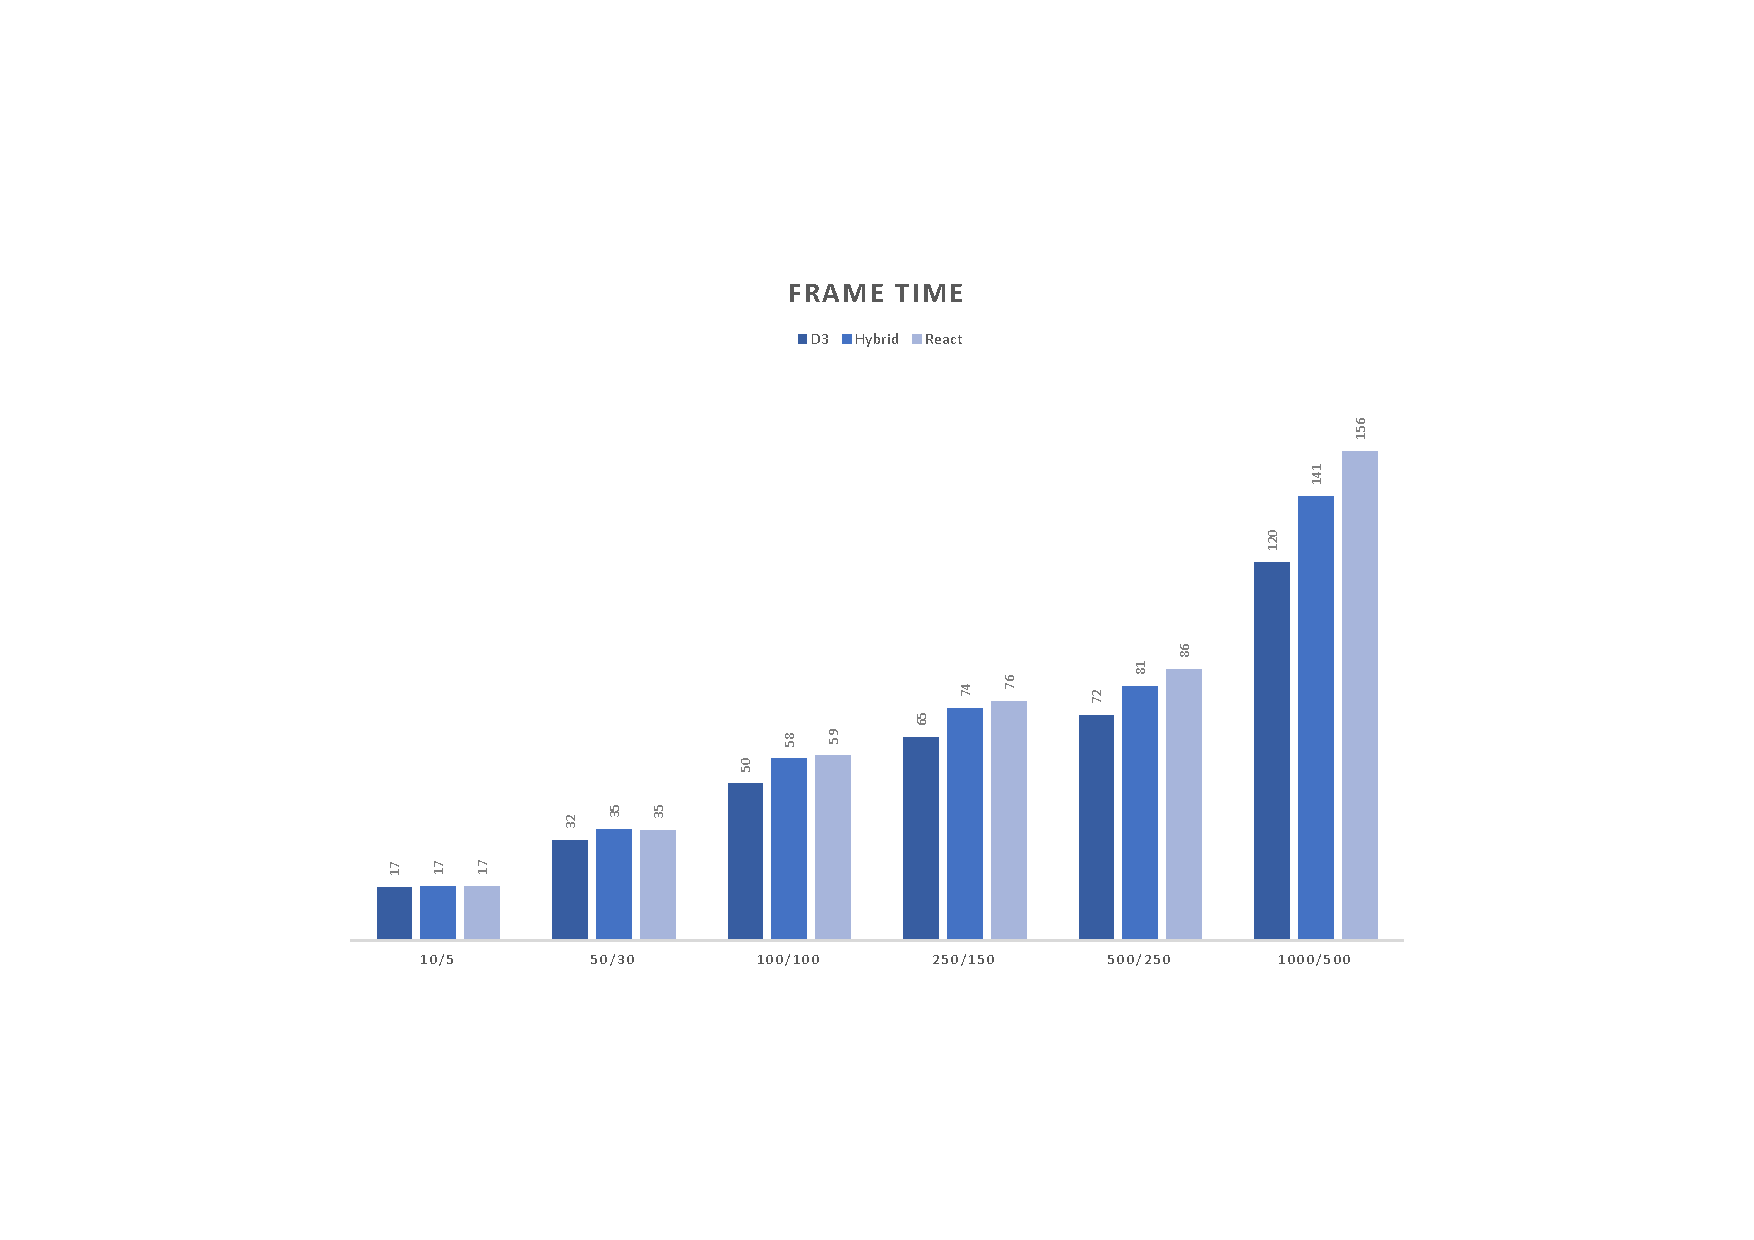
\includegraphics[scale=2.5, trim= 4cm 4.5cm 4cm 4.5cm, clip, width=1\columnwidth]{perfLowEnd003.pdf}
\caption{Low-end devices' average frame time per benchmark iteration cycle (lower is better).}
\label{fig:perfLowEnd003}
\end{figure}

Looking at the high-end results in figure~\ref{fig:perfHighEnd003} the same pattern as before can be observed, where the first iterations are capped to a specific minimum value. However, the rest of the results increase exponentially, which correlates to the rest of the high-end performance results. The average frame time of the last iteration stands out and spikes with an exceptionally high value.

\begin{figure}
\centering
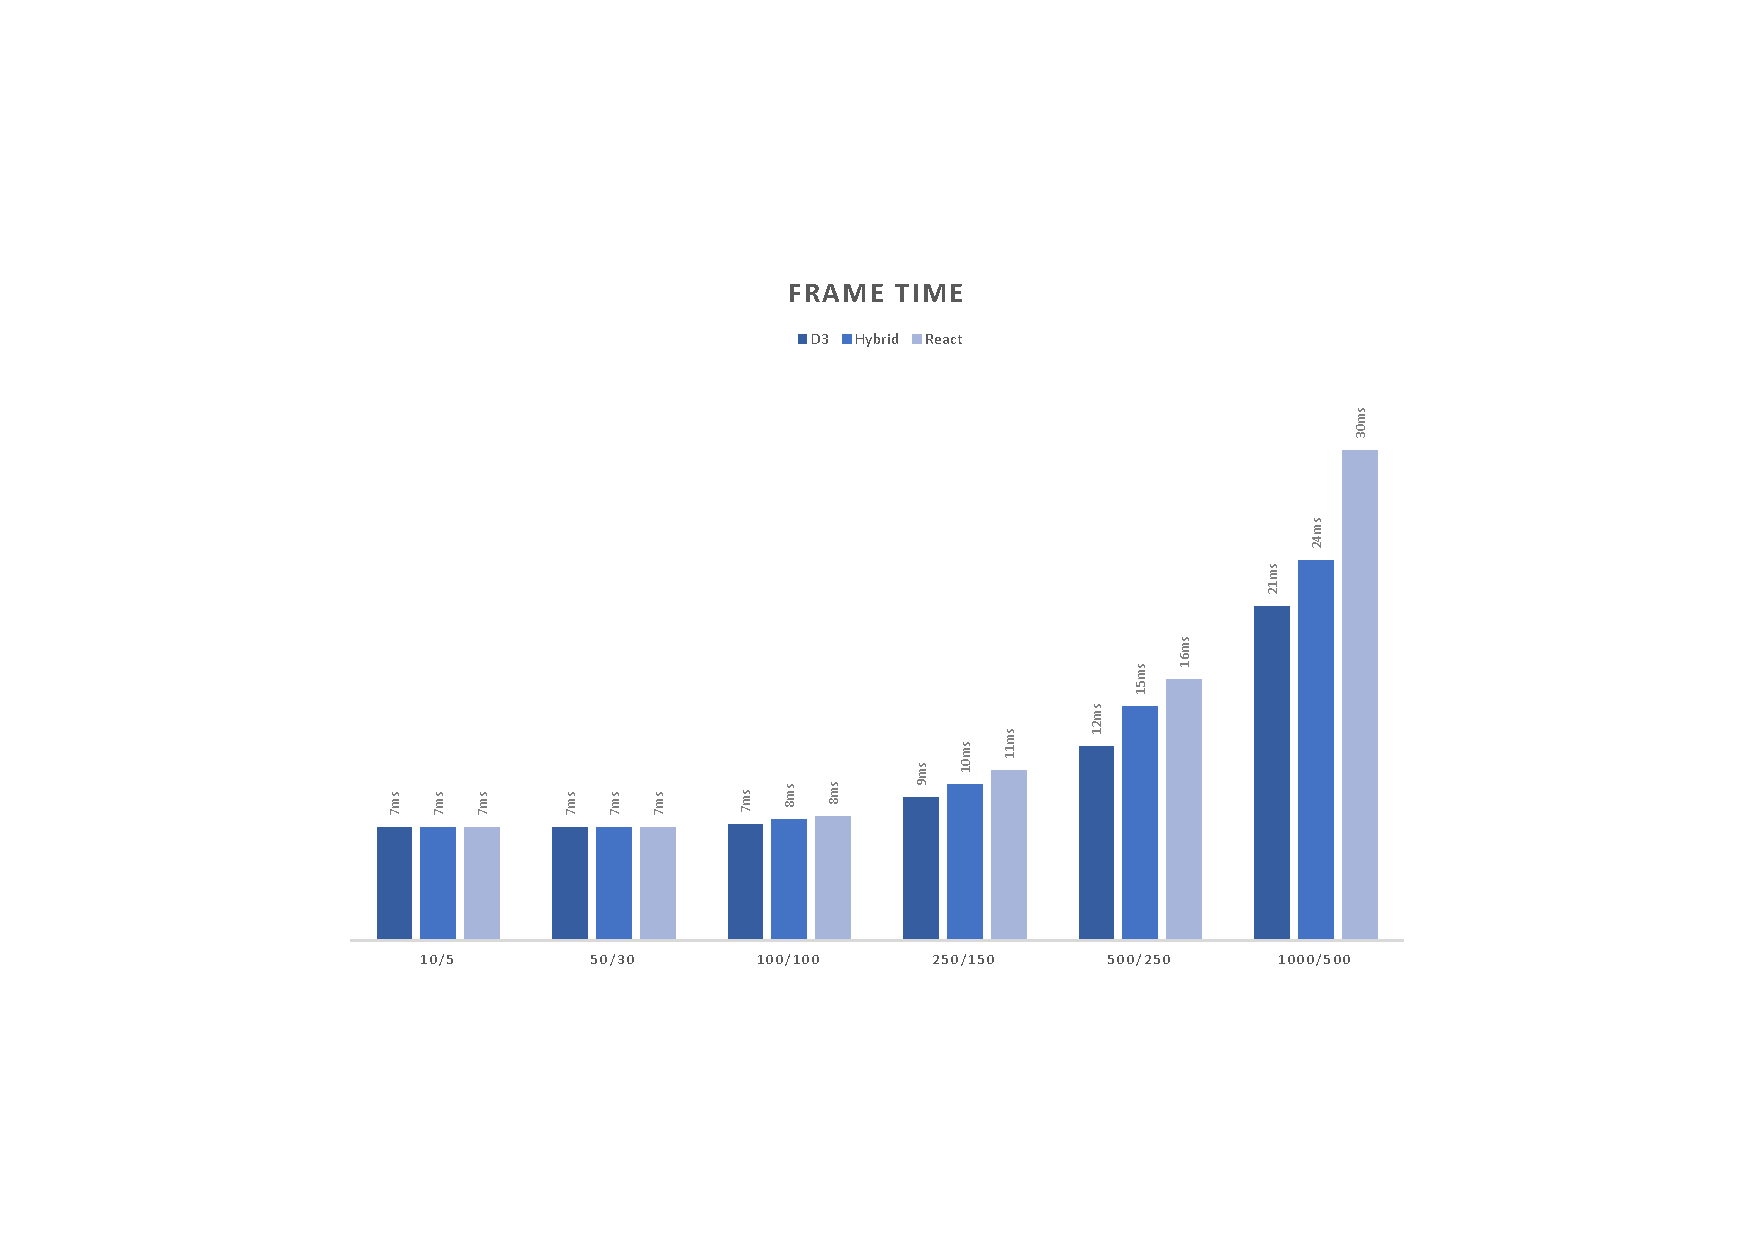
\includegraphics[scale=2.5, trim= 4cm 4.5cm 4cm 4.5cm, clip, width=1\columnwidth]{perfHighEnd003.pdf}
\caption{High-end devices' average frame time per benchmark iteration cycle (lower is better).}
\label{fig:perfHighEnd003}
\end{figure}

Last but not least, a critical aspect of any animation performance measurement is the maximum time between frames measured. The value can provide critical insights to some performance issues even though the average frame time per second might look okay. The chart in figure~\ref{fig:perfLowEnd004} shows an average of the maximum frame time value to each iteration cycle. One unanticipated result was that the maximum frame rate of the hybrid component is sig\-nifi\-cantly higher throughout the testing results than the pure \emph{D3} or pure \emph{React} components.

\begin{figure}
\centering
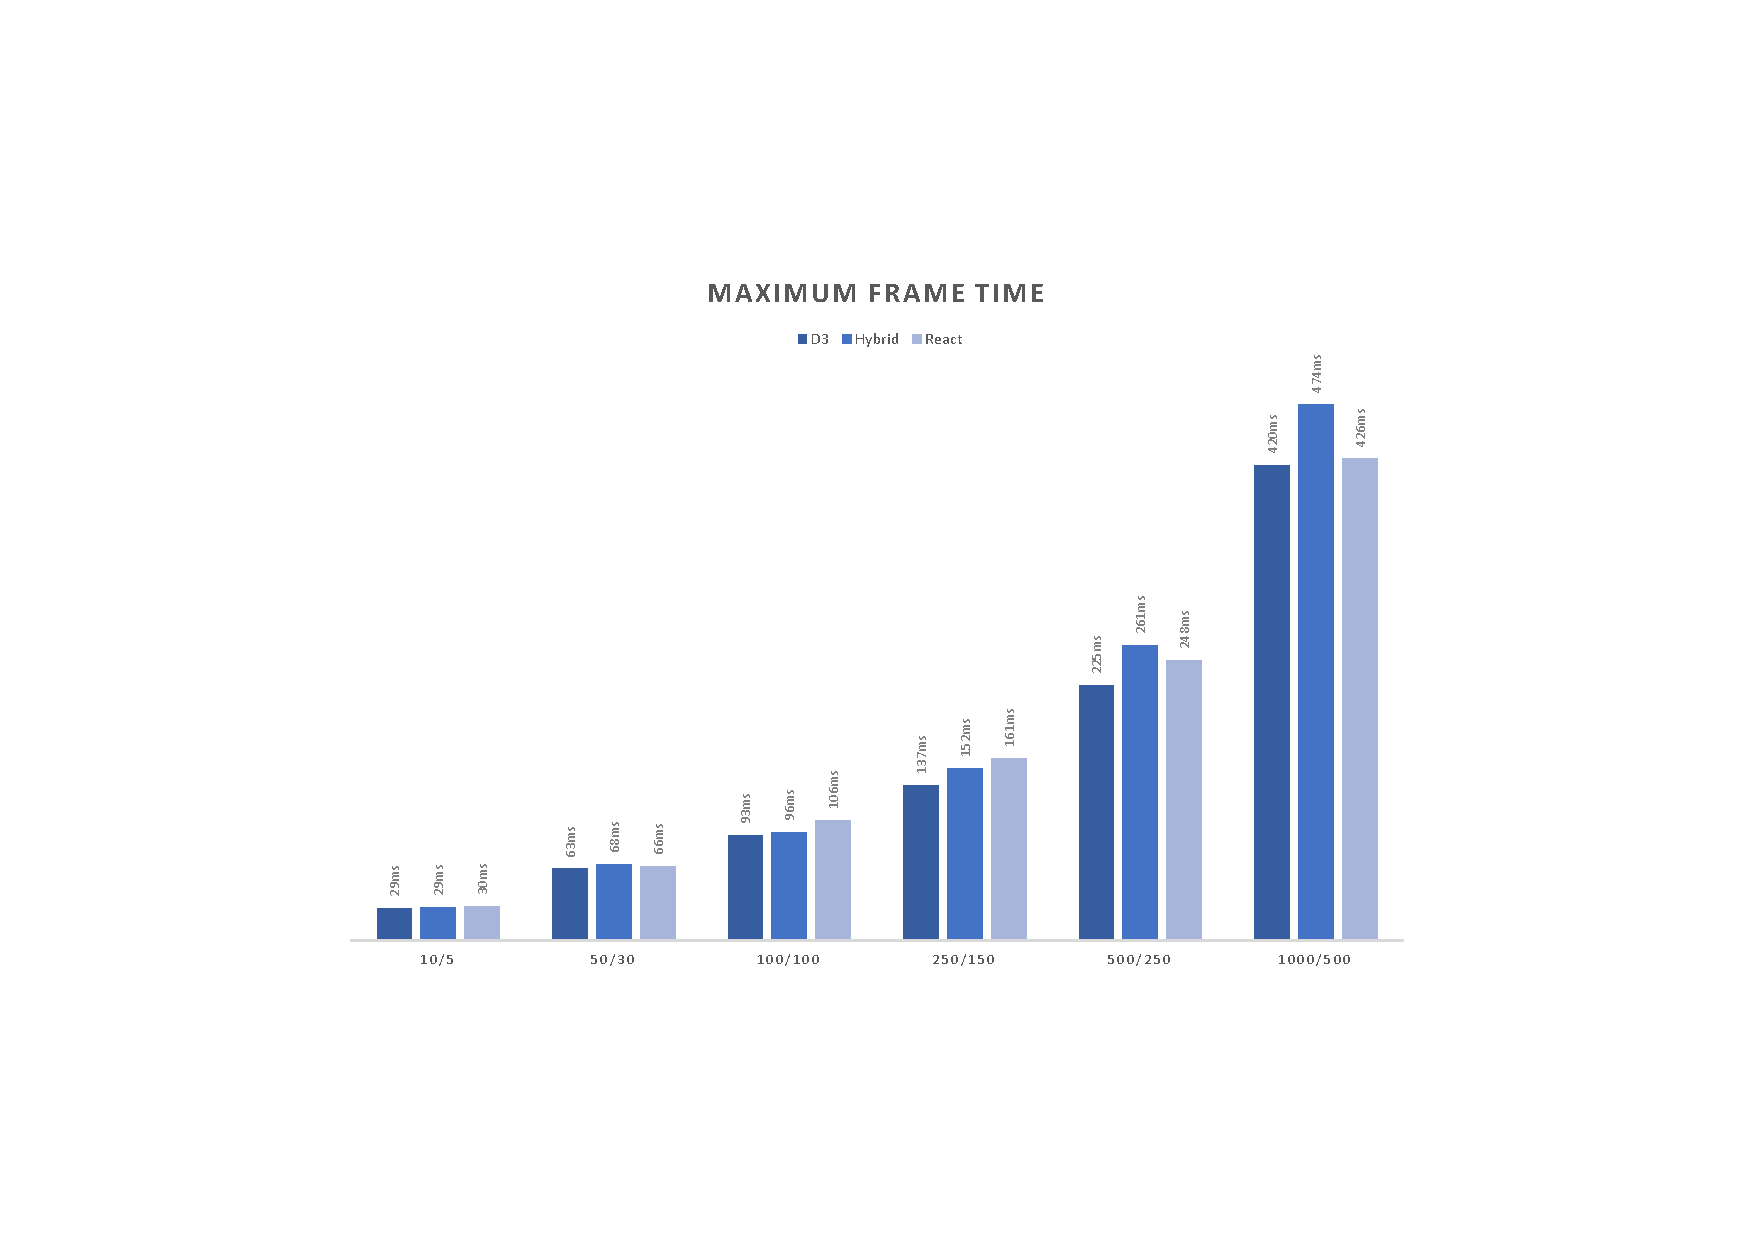
\includegraphics[scale=2.5, trim= 4cm 4.5cm 4cm 4.5cm, clip, width=1\columnwidth]{perfLowEnd004.pdf}
\caption{Low-end devices' average maximum frame time per benchmark iteration cycle (lower is better).}
\label{fig:perfLowEnd004}
\end{figure}

However, the performance graph in figure~\ref{fig:perfHighEnd004} shows the high-end devices' maximum frame time results which are more expected. Again, the average maximum frame time rises exponentially. The results contain a few irregularities, though. The maximum frame time of the reference pure \emph{D3} prototype, for example, is sometimes higher as the value of the other two prototypes. The maximum frame time values, therefore, must be taken with a grain of salt, as any maximum value could be caused by an unexpected system or browser activity which could have decreased the overall performance of any prototype. As mentioned before, the problem is mitigated by executing one iteration multiple times, but there is still a margin of error, though.

\begin{figure}
\centering
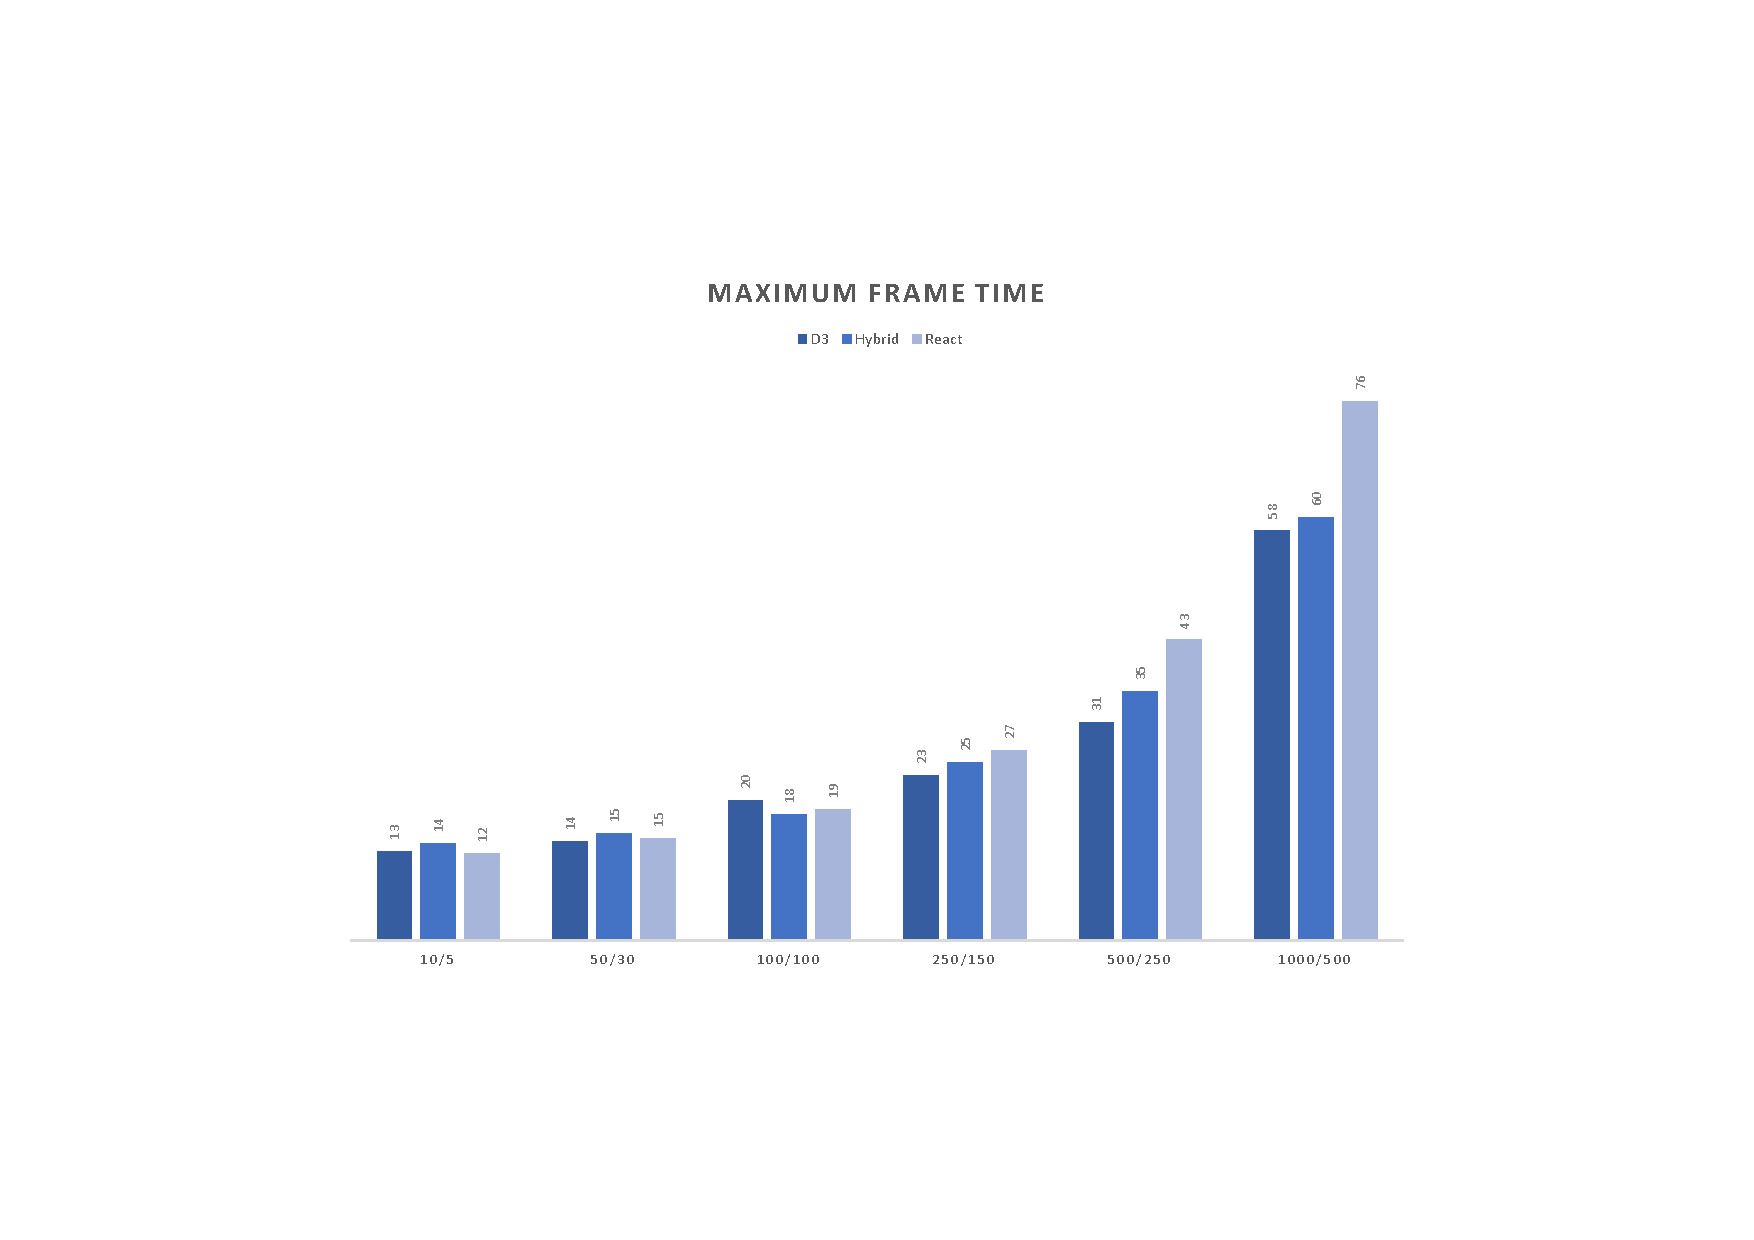
\includegraphics[scale=2.5, trim= 4cm 4.5cm 4cm 4.5cm, clip, width=1\columnwidth]{perfHighEnd004.pdf}
\caption{High-end devices' average maximum frame time per benchmark iteration cycle (lower is better).}
\label{fig:perfHighEnd004}
\end{figure}

\subsection{Human Perception of Fluent Animations}
\label{sub:humanPerception}

%%Humans vision is bad lol, they can only see 13 FPS but when do we actually notice some stuttering or laggy animation performance? 

Human vision is a very complicated topic, as there has been a large volume of studies over many years which tried to determine at which point humans perceive a series of images as fluent motion. Read \& Meyer claim in~\cite{RestorationOfMotionPictureFilm} that humans perceive motion if the animation is displayed with at least 12 frames per second. During further research, another article in~\cite{Potter2014} was found which states that humans can detect specific images in a rapid serial visual representation (RSVP) of a series of multiple pictures. The paper in~\cite{Potter2014} found that participants could determine if the RSVP stream contained a specific picture even with a frequency of displaying each picture for just 13ms. 

Another vital question is at which point an observer does not perceive an animation as fluent anymore. As mentioned before, the time per frame should be below 13ms in the best case to provide the perception of fluent animation. Although animations with at least 12 frames per second can be perceived as motion, they are not necessarily experienced as fluent motion though. As the performance measurements of the thesis project yield some final numbers, they can be used to determine if the animation of the test can be experienced as fluent motion or not.

Further research in the field of human perception of animation revealed yet another interesting result. Countless studies throughout the last decades have tried to find an answer to the question at which point humans do not experience an animation as stuttering or flickering anymore. Previous research has established that flickering or so-called "stuttering" cannot be detected if the human perception cannot distinguish between modulated light and a stable field anymore. The rate seems to be between 50 and 90 Hertz according to several resources in~\cite{6375944,farrell1987predicting,stereoscopicFlickerArticle}. Even though the findings are mostly about the refresh rate of monitors, the same principle also applies for the displayed frames per second of an animation rendered in the browser.

\subsection{Interpreting the Test Results}

When interpreting the test results, it is essential to keep in mind that the hybrid implementation uses a custom animation library internally, as mentioned in subsection~\ref{sub:D3AndReactHybrid} which can be turned off to improve performance. The animation feature was turned on during the execution of the benchmark tests even though the test iterations do not include any individual node animation. As a result, the pure \emph{React} component has a clear advantage over the hybrid component by not having to calculate node animations as they are not implemented on the pure \emph{React} component. Even though the additional performance decreasing feature was kept on during all tests, the hybrid component generally yielded equal or better performance numbers in comparison to the pure \emph{React} prototype.

Another clear advantage of the \emph{React} prototype is that newer versions of \emph{React} provide functionality which assigns a lower priority to DOM nodes which are outside the viewport of the browser. Lin Clark explains the functionality of the library during the \emph{React} conference in~\cite{ReactReconcliliationVideo}, where the feature was first introduced. Due to the fact that mobile devices mostly have smaller viewports, a large proportion of the nodes in higher iteration difficulties is rendered outside of the viewport again providing an advantage to the \emph{React} prototype.

Looking at the frames per seconds, the charts in figures~\ref{fig:perfLowEnd001} and~\ref{fig:perfHighEnd002} indicate how the \emph{D3} prototype yields the best result in every iteration, followed by the hybrid implementation with the second best results and lastly the pure \emph{React} prototype with the slowest results. Closer inspection of the two charts shows that the performance decrease is linear, whereas the increase of render difficulty in figure~\ref{fig:perfIterations} is exponential. Because the frames per second are calculated via the \texttt{requestAnimationFrame()} function, the results show that the browsers regularly try to provide animation frames even though the calculations get exponentially harder.

In comparison to the earlier presented results, the overall TTC values in figures~\ref{fig:perfLowEnd002} and~\ref{fig:perfHighEnd002} do not correlate with the frames per second which is a rather unexpected result. As mentioned before, browsers try to provide as many animation frames as possible, whereas the overall TTC is measured via two timestamps. A remarkable outcome though is the fact that the first and most lightweight iteration results show that the low-end devices' TTC is roughly 40\% of the high-end devices' TTC. This supports the theory that the monitor refresh rate is directly tied to the browsers' request animation frame functionality as 40\% of 144 roughly equals 60. 

The high-end and low-end TTC values do not correlate either. While the high-end benchmark values in figure~\ref{fig:perfHighEnd002} show the expected exponential increase of TTC, the low-end results in figure~\ref{fig:perfLowEnd002} show a linear increase for the TTC one iteration cycle. The findings can be explained that browsers cannot complete full render and paint cycles anymore during one animation frame due to the low-end hardware. By generating a constant backlog of due animation frames, some of them might get dropped due to new animation frame requests that are more recent. Once animation frames get canceled because of more recently requested animation frames, the pattern of increasing completion time is more comparable to the pattern of the overall FPS increase in the charts in figures~\ref{fig:perfLowEnd001} and~\ref{fig:perfHighEnd002}. The high-end results in figure~\ref{fig:perfHighEnd002} show the expected exponential increase of TTC an iteration cycle, as browsers can process the calculations completely within the requested animation frame.

Figures~\ref{fig:perfLowEnd003} and~\ref{fig:perfHighEnd003} show the average frame times of the prototypes. The results can be seen as another way to describe frames per second. As described in section~\ref{sub:humanPerception}, the frame times play a crucial role for humans to percieve an animation as fluent without stuttering. For all low-end devices, benchmarks showed rather high average frame times starting from the second benchmark iteration. While the results stayed well above the previously mentioned 12 frames per second threshold, the lower frame time is definitely noticeable. Probably one of the most sig\-nifi\-cant findings when looking at the general trend, the hybrid prototype regularly comes out ahead, when comparing the average frame times. The high-end chart in figure~\ref{fig:perfHighEnd003} shows a clear spike of the pure \emph{React} implementation in the last iteration. A possible explanation for this outcome might be that \emph{React} reaches the previously already mentioned threshold when performing the calculation for an animation frame. \emph{React} performs pretty well, considering it has to process 1500 DOM nodes every 30ms completely and put them through a complete render cycle.

Last but not least, the maximum frame time results can also provide valuable insights into how the prototypes perform compared to each other. These results must be interpreted with caution though, because various unforeseeable reasons can cause maximum frame time spikes. The results for the low-end devices in figure~\ref{fig:perfLowEnd004} show, for example, that the hybrid component had the highest maximum frame time in the last two iterations. Now, if this only happens once in the animation, this might not be noticeable, but if this would be a continuous trend, the data could point to a performance problem in the implementation of the prototype. The explanation for the performance spikes is most likely also tied to the fact that low-end devices run into the animation frame limit of not being able to calculate a full render cycle in one animation frame. The hybrid component not only has to build up the whole component tree via react but also calculate the animations with react move. If both instances are limited to animation frame constraints, the calculation could be spread out across multiple frames, making the whole animation slower in the process.

On the contrary, the high-end maximum frame time tests in figure~\ref{fig:perfHighEnd004} yield more expected results. When having to deal with many nodes and links, the maximum frame times should be equally affected as a consequence. The last iteration shows the longest time between frames for the pure \emph{React} prototype, which is 76 milliseconds. The pure \emph{D3} and hybrid component seem to be able to maintain a maximum frame time at about 60 milliseconds during the cycles of the last iteration.

%Generally a correlation between the time to complete, average frame time and the maximum frame time can be observed when looking at all the charts again.

\section{Conclusion}

All in all, the different prototypes performed quite well in general. The question "Why does the benchmark use numbers as high as 1000 nodes and 500 links?" which might come up during the examination of the testing results can quickly be answered. The test that was used to benchmark the prototypes uses a simple force simulation configuration where each base node is just a single circle element, and each link is a path element. When using more sophisticated nodes which contain multiple SVG elements, the outcome could be the same. If an example simulation would use ten SVG elements in just one node, rendering 100 of those nodes would yield a similar outcome as rendering the 6th benchmark iteration.

Overall all the prototypes performed pretty well. As mentioned before, the pure \emph{D3} component is the clear winner and best performing prototype, but that was the expected result, as it was developed to serve as a baseline for the results of the other prototypes. When glancing over the rest of the results, the hybrid nearly always comes out ahead of the pure \emph{React} prototype. The primary purpose of the study was if \emph{React} can be combined with \emph{D3} without losing performance in the browser. The definitive answer to that question has to be no, unfortunately, as there are some performance penalties when combining two full grown libraries. The test results also support the answer to the research question.

When talking about user experience though, the prototypes are pretty much all usable in production projects, as the divergence of the performance numbers mostly stays within the bounds of a smooth animation experience. The benchmark results of the third and fourth iteration are acceptable when looking at the FPS and average frame time. When using the force graphs on mobile devices, the performance is worse overall, but due to the fact that even the pure \emph{D3} prototypes performed a lot worse on low-end devices, the combination prototypes cannot magically yield a better performance, as they technically not only have to calculate \emph{D3} force simulation ticks but also \emph{React} render cycles. As a consequence, the performance is worse than just letting \emph{D3} handle the whole simulation on its own. 

